\documentclass[11pt]{article}
\usepackage[T1]{fontenc}
\usepackage{lmodern,microtype,amsmath,amssymb,amsthm,booktabs,graphicx}
\usepackage[margin=1.04in]{geometry}
\usepackage[colorlinks=true,linkcolor=blue!45!black,urlcolor=blue!45!black,citecolor=blue!45!black]{hyperref}
\usepackage{xcolor}
\newtheorem{theorem}{Theorem}
\newtheorem{lemma}[theorem]{Lemma}
\newtheorem{corollary}[theorem]{Corollary}
\newcommand{\norm}[1]{\lVert #1\rVert_\infty}
\newcommand{\dd}{d_{\mathrm L}}
\title{\bfseries The minimum Lorentz degree for polynomials\\ with all zeros in a thin ellipse}
\author{Research note}
\date{November 27, 2026}
\begin{document}
\maketitle
\begin{abstract}
In 1991 Erd\'elyi asked whether confining every zero of a degree-$n$ polynomial to the open ellipse of semiaxes $1,\varepsilon$ forces its Lorentz degree to be at least $cn/\varepsilon^2$. We determine the correct order for each even $n\ge2$ and each $0<\varepsilon\le1$. The minimum finite Lorentz degree is comparable to $\max\{n/\varepsilon,\varepsilon^{-2}\}$ with absolute constants. Rational polynomials with simple zeros attain the upper order. A scaled Chebyshev polynomial gives explicit counterexamples to the proposed bound. Two independent inequalities give the lower order: a logarithmic integral on confocal ellipses counts the contribution of many roots, and convexity on the real axis isolates a single extreme root.
\end{abstract}

\section{The question and the counterexample}
A Lorentz representation on $[-1,1]$ is a polynomial identity
\[
   P(x)=\sum_{j=0}^{D} a_j(1-x)^j(1+x)^{D-j}
\]
in which all $a_j$ have the same weak sign. Its least possible degree is $\dd(P)$. If $P$ is strictly positive on $[-1,1]$, all the coefficients of any such representation are nonnegative. Let
\[
 \mathcal E_\varepsilon=\{x+iy:x^2+y^2/\varepsilon^2<1\},\qquad 0<\varepsilon\le1.
\]
In Section 8, page 197 of his 1991 paper, Erd\'elyi asks whether a universal $c>0$ gives $\dd(P)\ge c n/\varepsilon^2$ for \emph{every} real polynomial of degree $n$ with all its zeros in $\mathcal E_\varepsilon$ \cite{erd}. His paper also establishes large Lorentz degrees for powers of particular quadratics. The ellipse question concerns arbitrary distributions of the zeros.

Let $L_n(\varepsilon)$ be the least finite Lorentz degree among polynomials of ordinary degree $n$ with all roots in $\mathcal E_\varepsilon$. A real polynomial of odd degree has a real root. If all its roots lie in this ellipse, that root belongs to $(-1,1)$, where a nonzero polynomial with a same-sign Lorentz representation cannot vanish. The finite problem thus has even $n$.

\begin{theorem}[The joint extremal order]\label{joint}
For every even $n\ge2$ and every $0<\varepsilon\le1$, put
$M_n(\varepsilon)=\max\{n/\varepsilon,1/\varepsilon^2\}$. Then
\begin{equation}\label{answer}
 \boxed{\qquad \frac{3}{100}M_n(\varepsilon)\ \le\ L_n(\varepsilon)\
              \le\ 513M_n(\varepsilon).\qquad}
\end{equation}
The upper bound holds with simple zeros and rational coefficients. In the range $n\varepsilon>4$ its constant may be taken to be $64$.
\end{theorem}

Theorems~\ref{universal} and \ref{widthcost} give the two lower estimates, and Theorem~\ref{jointupper} gives the constructions. The examples below already decide the original yes-or-no question.

\begin{theorem}\label{main}
For $n=4,8,12,\ldots$, put $s_n=1+n^{-2}$ and
\[
                  P_n(x)=2+T_n(s_nx), \qquad \varepsilon_n=2/n,
\]
where $T_n(\cos\theta)=\cos(n\theta)$. Then $P_n\in\mathbb Q[x]$ has degree $n$, is strictly positive on $[-1,1]$, and has $n$ distinct zeros in $\mathcal E_{\varepsilon_n}$. Furthermore
\begin{equation}\label{bound}
              \frac{s_n^2 n^2}{3}\ \le\ \dd(P_n)\ \le\ 8 n^2 .
\end{equation}
\end{theorem}

In particular $\varepsilon_n^2\dd(P_n)/n\le32/n\longrightarrow0$. The same family defeats every proposed lower bound $c_\alpha n/\varepsilon^\alpha$ with fixed $\alpha>1$. Multiplying $P_n$ by a positive common denominator gives examples with integer coefficients and the same zeros and Lorentz degree.

\section{Where all the roots lie}
Write $a=\operatorname{arcosh}2$, so $\sinh a=\sqrt3$. The $n$ roots are
\begin{equation}\label{roots}
 z_j=s_n^{-1}\cos\!\left(\frac{(2j+1)\pi}{n}+i\frac an\right),
                 \qquad 0\le j<n.
\end{equation}
Indeed, applying $T_n$ multiplies the argument by $n$ and gives $-\cosh a=-2$. The map $\theta\mapsto\cos(\theta+i a/n)$ is an injective parametrization modulo $2\pi$ of an ellipse, so the listed zeros are distinct. The recurrence of the Chebyshev polynomials gives rational coefficients and degree $n$.

The semiaxes of the ellipse in \eqref{roots} are $A_n=\cosh(a/n)/s_n$ and $B_n=\sinh(a/n)/s_n$. Termwise comparison of the hyperbolic series gives
\[
 \cosh(a/n)<1+\frac{\cosh a-1}{n^2}=s_n,\qquad
 \sinh(a/n)\le\frac{\sinh a}{n}=\frac{\sqrt3}{n}.
\]
Consequently $A_n<1$ and $B_n<2/n$. Each root satisfies the required \emph{strict} ellipse inequality.
For $|s_n x|\le1$ we have $P_n(x)\ge1$. For $|s_nx|\ge1$ the evenness of $n$ and the hyperbolic formula give $T_n(s_nx)\ge1$. On $[-1,1]$ we also have
\begin{equation}\label{sup}
 \norm{T_n(s_n\,\cdot)}\le T_n(s_n)
 =\cosh(n\operatorname{arcosh}(1+n^{-2}))\le\cosh\sqrt2<9/4 .
\end{equation}
Here $\cosh v\ge1+v^2/2$. For the last bound, the terms in $\cosh\sqrt2$ starting at degree four sum to at most $(1/6)/(1-1/15)$.

\begin{center}
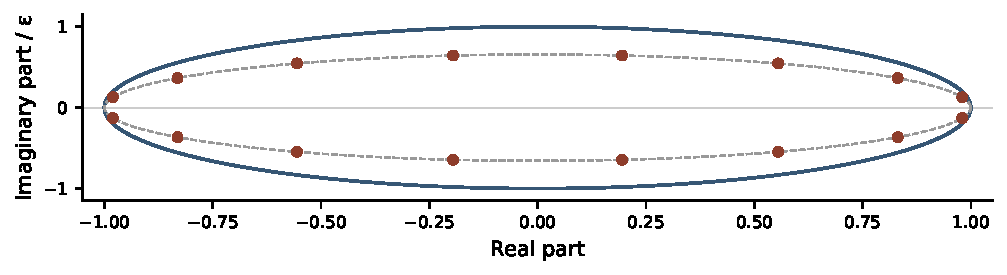
\includegraphics[width=.90\linewidth]{ellipse_zeros.pdf}
\end{center}
\noindent\small For $n=16$ the red points are all sixteen roots. The dashed ellipse contains them on its boundary. The outer ellipse is $\partial\mathcal E_{2/n}$. The vertical coordinate is divided by $\varepsilon$.\normalsize

\section{A uniform upper bound for the positive representation}
On $[0,1]$ let $B_D$ be the Bernstein operator
\[
   B_D f(t)=\sum_{j=0}^{D} f(j/D){D\choose j} t^j(1-t)^{D-j}
           =\mathbb E[f(K/D)],\qquad K\sim{\rm Binomial}(D,t).
\]
It maps the space of polynomials of degree at most $n\le D$ into itself. This follows by expanding a polynomial in the falling factorials of $K$, whose expectations are $(D)_j t^j$.

\begin{lemma}\label{operator}
On the space of polynomials of degree at most $n\le D$, with supremum norm on $[0,1]$,
\[
             \|I-B_D\|\le 2n^2/D.
\]
If $\eta=2n^2/D<1$, then $B_D$ is invertible on this space and $\|B_D^{-1}-I\|\le\eta/(1-\eta)$.
\end{lemma}
\begin{proof}
If $\deg f\le n$, let $g(\theta)=f((1+\cos\theta)/2)$ and put $t=(1+\cos\theta)/2$. Differentiation gives
\[
 g''(\theta)=t(1-t)f''(t)-\tfrac12(2t-1)f'(t).
\]
Twice applying Bernstein's trigonometric inequality \cite{bern} gives $\norm{g''}\le n^2\norm f$, and Markov's inequality on $[0,1]$ gives $\norm{f'}\le2n^2\norm f$. Consequently
\[
 H:=\sup_{0<t<1}t(1-t)|f''(t)|\le2n^2\norm f .
\]
Set $h(t)=t\log t+(1-t)\log(1-t)$, continuously extended to $[0,1]$. Since $h''(t)=1/[t(1-t)]$, the functions $Hh\pm f$ are convex. Applying their tangent inequalities at $0<t<1$ yields for $0\le u\le1$
\[
 |f(u)-f(t)-(u-t)f'(t)|\le H\left[u\log\frac ut+(1-u)\log\frac{1-u}{1-t}\right].
\]
Zero times its logarithm is interpreted as zero. The bracket is at most $(u-t)^2/[t(1-t)]$ by $\log x\le x-1$. For $U=K/D$ with $K\sim{\rm Binomial}(D,t)$, take expectations and use $\mathbb E U=t$ and $\operatorname{Var}(U)=t(1-t)/D$. At $t=0,1$ the operator error vanishes. We have proved
\begin{equation}\label{weightedop}
 \|I-B_D\|\le2n^2/D
\end{equation}
on the polynomials of degree at most $n$. The Neumann series gives the asserted inverse estimate.
\end{proof}

Set $D=8n^2$, $g_n(t)=T_n(s_n(2t-1))$ and $F_n=2+g_n$. By the lemma, $\eta=1/4$. Equation \eqref{sup} and $B_D1=1$ give
\[
 \norm{B_D^{-1}F_n-F_n}\le\frac{\eta}{1-\eta}\norm{g_n}<\frac34 .
\]
Since $F_n\ge1$, every value $(B_D^{-1}F_n)(j/D)$ is strictly positive. Substituting these values into the definition of $B_D$ gives $F_n$ exactly. With $t=(1+x)/2$, the resulting Bernstein representation is a degree-$D$ Lorentz representation of $P_n$. This proves the upper bound without a limiting argument in an auxiliary power.

\section{A lower bound at a single point}
For $h_j(x)=(1-x)^j(1+x)^{D-j}$ one has
\[
          h_j(0)=1,\qquad h_j''(0)=(D-2j)^2-D.
\]
Thus every polynomial $P>0$ with a degree-$D$ Lorentz representation satisfies
$P''(0)\ge-DP(0)$. For $4\mid n$, $T_n(0)=1$, and the Chebyshev differential equation
$(1-x^2)T_n''-xT_n'+n^2 T_n=0$ yields $T_n''(0)=-n^2$.
Now $P_n(0)=3$ and $P_n''(0)=-s_n^2n^2$. The lower bound in \eqref{bound} follows.

\section{The universal lower bound}

\begin{theorem}\label{universal}
Let $0<\varepsilon\le 1$ and let $p$ be a real polynomial of ordinary degree $n\ge 1$ with every root in $\mathcal E_\varepsilon$. If $p$ admits a Lorentz representation on $[-1,1]$, then
\[
                  \dd(p)\ \ge\ \frac{n}{16\varepsilon}.
\]
\end{theorem}
\begin{proof}
Changing the sign of $p$ if necessary, write
\[
 p(X)=\sum_{j=0}^D b_j(1-X)^j(1+X)^{D-j},\qquad b_j\ge 0,\qquad D=\dd(p).
\]
The open ellipse excludes $\pm1$, so $p$ is strictly positive on $[-1,1]$. If $\varepsilon\ge1/16$, then $D\ge n$ gives the result. Hence assume $\varepsilon<1/16$ and put $v=4\varepsilon<1/4$.

For $w\in\mathbb C$, define $g(w)\ge0$ as the logarithm of the larger of the two moduli of the roots of $Z^2-2wZ+1=0$. The roots have product one. The set $\{g\le t\}$ for $t>0$ is the closed ellipse with semiaxes $\cosh t,\sinh t$ and foci $\pm1$: the parametrization $w=(Z+Z^{-1})/2$ with $Z=e^{t+i\theta}$ gives its boundary, and the ellipses are nested as $t$ increases. For each $t\ge0$,
\begin{equation}\label{ell-jensen}
 \frac1{2\pi}\int_0^{2\pi}\log|\cos(\theta+it)-w|\,d\theta
       =-\log 2+\max(t,g(w)).
\end{equation}
Indeed the circle $|Z|=e^t$ parametrizes the same ellipse with uniform angle (up to reversal). Factor $(Z+Z^{-1})/2-w=(Z-Z_1)(Z-Z_2)/(2Z)$. The circle mean of $\log|Z-Z_j|$ is $\log\max(e^t,|Z_j|)$ by Jensen's formula; the identity also holds at equality by the integrability of the logarithmic singularity. Substitution gives \eqref{ell-jensen}.

For real $\theta$ the exact identities $|1\pm\cos(\theta+iv)|=\cosh v\pm\cos\theta$ and $b_j\ge0$ imply
\[
 |p(\cos(\theta+iv))|\le (\cosh v)^D\,p(\cos\theta/\cosh v).
\]
Take logarithms and integrate. Apply \eqref{ell-jensen} on the left to each root $\zeta$ of $p$ at $t=v$, counted with multiplicity. On the right use $t=0$ and $w=(\cosh v)\zeta$, extracting $(\cosh v)^{-1}$ from each linear factor. The leading coefficient cancels and we obtain
\begin{equation}\label{ell-budget}
 \sum_{p(\zeta)=0}\bigl[\max(v,g(\zeta))-g((\cosh v)\zeta)\bigr]
          \le (D-n)\log\cosh v.
\end{equation}

Every term on the left is nonnegative. Indeed $\varepsilon=v/4\le\tanh v$ in the stated range, so the ellipse $(\cosh v)\mathcal E_\varepsilon$ lies inside $\{g\le v\}$ by comparing both semiaxes. A root $\zeta=x+iy$ satisfying $1-x^2\ge 4v^2$ gives a term of at least $v/2$. To verify this, put
\[
 A=\frac{\cosh^2 v}{\cosh^2(v/2)},\qquad
 B=\frac{\varepsilon^2\cosh^2 v}{\sinh^2(v/2)} .
\]
We have $A\ge1$, $A-1\le\sinh^2v\le2v^2$, and $B\le\cosh^2 v/4\le1/2$, using $v\le1/4$, $\sinh(v/2)\ge v/2$ and $\sinh v\le v\cosh v$. The ellipse hypothesis gives $y^2\le\varepsilon^2(1-x^2)$. Consequently
\[
 \frac{(\cosh v)^2x^2}{\cosh^2(v/2)}
 +\frac{(\cosh v)^2y^2}{\sinh^2(v/2)}
 \le A-(A-B)(1-x^2)
 \le 1+2v^2-\tfrac12(1-x^2)\le1 .
\]
This means $g((\cosh v)\zeta)\le v/2$. If at least $n/2$ roots satisfy the displayed condition, \eqref{ell-budget} and $\log\cosh v\le v^2/2$ yield $D-n\ge n/(2v)$.

Otherwise more than $n/2$ roots satisfy $1-x^2<4v^2$. After reflecting $p(X)$ to $p(-X)$ if needed, at least $n/4$ roots have $x\ge0$ and $1-x\le 1-x^2<4v^2$. Reflection preserves the degree and interchanges the Bernstein coefficients. Differentiating the representation at $1$ and using $b_0>0$ gives
\[
 D\ \ge\ 2\frac{p'(1)}{p(1)}
    =2\sum_{p(\zeta)=0}\frac{1-x}{(1-x)^2+y^2}.
\]
Every summand is positive since $x<1$. Moreover $y^2\le 2\varepsilon^2(1-x)$. For each of the selected roots the summand is therefore at least
$1/(1-x+2\varepsilon^2)\ge 1/(5v^2)$. This yields $D\ge n/(10v^2)\ge n/(4v)$ because $v\le 1/4$. Both cases give $D\ge n/(4v)=n/(16\varepsilon)$.
\end{proof}
\section{A bound forced by one extreme root}
There is a second cost when the ellipse is especially thin compared to the degree. It can be seen on the real axis through the curvature of the logarithm of $P$.

\begin{theorem}\label{widthcost}
Under the hypotheses of Theorem~\ref{universal}, one has
\[
                          \dd(P)\ge \frac{3}{100\varepsilon^2}.
\]
\end{theorem}
\begin{proof}
Take the positive sign of $P$ and write $D=\dd(P)$. For real $s$, the function
\[
    (\cosh s)^D P(\tanh s)=\sum_{j=0}^D a_j e^{(D-2j)s}
\]
has convex logarithm. Its second logarithmic derivative is the variance of $D-2j$ under the probabilities proportional to $a_j e^{(D-2j)s}$. Differentiation, with $x=\tanh s$, gives
\begin{equation}\label{curvature}
 D\ \ge\ \sum_{P(\zeta)=0}
       \left[(1-x^2)\operatorname{Re}\frac{1}{(x-\zeta)^2}
                 +2x\operatorname{Re}\frac{1}{x-\zeta}\right]
       \qquad (-1<x<1).
\end{equation}
All roots throughout the proof are counted with multiplicity.

Reflect the polynomial if necessary so that its leftmost root $\zeta_0=u+iy$ has $u\le0$, and set $h=1+u>0$. If $h\le32\varepsilon^2$, the left-endpoint version of the derivative bound in Theorem~\ref{universal} gives
\[
 D\ge-2P'(-1)/P(-1)=2\sum_\zeta\operatorname{Re}\frac{1}{1+\zeta}
   \ge\frac{2h}{h^2+y^2}\ge\frac{2}{h+2\varepsilon^2}
   \ge\frac{1}{17\varepsilon^2}.
\]
Here all terms are positive and $y^2\le\varepsilon^2(1-u^2)\le2\varepsilon^2 h$.

Suppose $h>32\varepsilon^2$. Put $\delta=2\varepsilon\sqrt{1-u^2}$ and $x=u-\delta$. Since $h\le1-u^2\le2h$, we have $\varepsilon^2\le\delta\le h/2$. Hence $-1<x<0$ and
$1-x^2\ge1+x\ge h/2\ge(1-u^2)/4$. For an arbitrary root $v+iw$ put $b=v-u\ge0$. The ellipse gives
\[
 w^2\le\varepsilon^2(1-v^2)
     \le\varepsilon^2(1-u^2+2b)\le(\delta+b)^2 .
\]
It follows that $\operatorname{Re}(x-\zeta)^{-2}\ge0$ and $x\operatorname{Re}(x-\zeta)^{-1}\ge0$ for every root. All contributions in \eqref{curvature} therefore have the same weak sign. For the selected extreme root, $|y|\le\delta/2$, so its first term alone gives
\[
 D\ge (1-x^2)\frac{\delta^2-y^2}{(\delta^2+y^2)^2}
       \ge \frac{1-u^2}{4}\cdot\frac{12}{25\delta^2}
       =\frac{3}{100\varepsilon^2}.
\]
This also holds in the endpoint case.
\end{proof}
\section{Examples at every degree and width}

\begin{theorem}\label{jointupper}
For each even $n\ge2$ and each $0<\varepsilon\le1$ there exists a degree-$n$ polynomial $p$ with rational coefficients and simple zeros all in $\mathcal E_\varepsilon$ for which
\[
 \dd(p)\le
 \begin{cases}
  513/\varepsilon^2,&n\varepsilon\le4,\\
  64n/\varepsilon,&n\varepsilon>4.
 \end{cases}
\]
\end{theorem}

\begin{proof}
Suppose first $n\varepsilon\le4$. Put $s=1+\varepsilon^2/4$, $a=\varepsilon/2$, and $P(X)=\cosh(na)+T_n(sX)$. Its zeros are
$s^{-1}\cos((2j+1)\pi/n+ia)$ for $0\le j<n$. Their ellipse has semiaxes $\cosh(a)/s<1$ and $\sinh(a)/s<\varepsilon$. Indeed, termwise comparison gives $\cosh(\varepsilon/2)-1\le\varepsilon^2(\cosh(1/2)-1)<\varepsilon^2/4$ and $\sinh(\varepsilon/2)\le\varepsilon\sinh(1/2)<\varepsilon$. Thus all roots lie strictly inside $\mathcal E_\varepsilon$. Evenness of $n$ gives $P(X)\ge\cosh(na)-1\ge n^2\varepsilon^2/8$ on $[-1,1]$. Also
\[
 \norm{T_n(s\,\cdot)}\le\cosh(n\operatorname{arcosh}(1+\varepsilon^2/4))
       \le\cosh(n\varepsilon/\sqrt2)\le\cosh(2\sqrt2)<9.
\]
Take $D=\lceil512/\varepsilon^2\rceil$ and $\eta=2n^2/D\le1/16$. Let $F(t)=P(2t-1)$. Since $B_D$ fixes constants, Lemma~\ref{operator} gives
\[
 \norm{B_D^{-1}F-F}\le\frac{\eta}{1-\eta}\norm{T_n(s\,\cdot)}
       \le \frac{36n^2}{D}<\frac{n^2\varepsilon^2}{8}.
\]
Every grid value of $B_D^{-1}F$ is strictly positive. Hence $P$ has a strictly positive Lorentz representation of degree $D\le513/\varepsilon^2$.

Suppose now $n\varepsilon>4$. Choose $m=2\max(2,\lceil1/\varepsilon\rceil)$, so $2/\varepsilon\le m\le4/\varepsilon<n$. Partition $n$ into even integers $b$ with $m\le b<2m$: use $\lfloor n/m\rfloor$ copies of $m$ and add the even remainder to one of them. For every such $b$, the root-location and upper-bound proofs of Theorem~\ref{main} apply to $P_b=2+T_b((1+b^{-2})X)$, since they require only that $b$ be even. All its roots belong to $\mathcal E_{2/b}\subseteq\mathcal E_\varepsilon$, and it has strictly positive Lorentz coefficients at degree $8b^2$. Multiplying these representations gives a polynomial of degree $n$ with all roots in $\mathcal E_\varepsilon$ and strictly positive Lorentz coefficients at degree
\[
                \sum_b8b^2\le16mn\le64 n/\varepsilon.
\]

In both constructions confinement to the open ellipse persists under sufficiently small perturbations of the ordinary coefficients, by continuity of the roots as a multiset. The coefficients in a fixed-degree Lorentz basis are linear in the ordinary coefficients, so strict positivity persists too. In this open neighborhood of the degree-$n$ polynomial there is a rational coefficient vector with nonzero discriminant: the discriminant is a nonzero polynomial on coefficient space and the rationals are dense. This gives the claimed simple roots and rational coefficients.
\end{proof}

\section{Exact checks and the positive-filter connection}
The least degrees in the table were determined in integer arithmetic. Put
$Q_n(z)=(n^2)^n(1+z)^nP_n((1-z)/(1+z))$. For $D\ge n$, a Lorentz representation of degree $D$ exists exactly when all coefficients of $(1+z)^{D-n}Q_n(z)$ are nonnegative. This equivalence follows by multiplying the defining representation by $(1+z)^D$ after the substitution. The coefficients in that basis are unique. Once they are all nonnegative, one further multiplication by $1+z$ preserves the property.
\begin{center}
\begin{tabular}{rrrr}
\toprule $n$ & $\dd(P_n)$ & $\dd(P_n)/n^2$ & $\varepsilon_n^2\dd(P_n)/n$\\\midrule
4 & 15 & .937500 & .937500\\
8 & 56 & .875000 & .437500\\
16 & 221 & .863281 & .215820\\
32 & 880 & .859375 & .107422\\
64 & 3516 & .858398 & .053650\\\bottomrule
\end{tabular}
\end{center}
The included script checks both $\dd(P_n)$ and $\dd(P_n)-1$. If $Q_n(z)=\sum_i q_i z^i$, the sign of coefficient $j$ after degree elevation is the sign of the integer
$\sum_i q_i(j)_i(D-j)_{n-i}$, with $(x)_k$ the falling factorial. The numerical values play no role in the proof.

The connection to the ProveIt article is algebraic. Its section on reflection-paired filters \cite{repo} characterizes sharp support by coefficientwise nonnegativity of a polynomial with prescribed roots. A central root supplies factors $1+z$. Under the preceding change of variable, adding exactly the same factor raises the allowed degree of a Lorentz representation by one. The root locations in \eqref{roots} spread the oscillations over the entire interval while the polynomial stays bounded above and bounded away from zero. The binomial operator then controls the cost of achieving positive coefficients. This argument is unconditional.

Erd\'elyi's article also poses two questions about products on the same page. Ait-Haddou treated those product bounds in 2015 \cite{ait}. The theorem here answers the thin-ellipse question. A targeted literature search found no earlier resolution of that question; historical priority would require a wider bibliographic review.

\paragraph{Further questions.}
What are the best constants in \eqref{answer}? Is there a limiting profile for $\varepsilon^2L_n(\varepsilon)$ as $n\to\infty$, $\varepsilon\downarrow0$ and $n\varepsilon$ approaches a fixed positive value? Even for the explicit family, the existence and value of $\lim_{4\mid n,\ n\to\infty}\dd(P_n)/n^2$ remain to be established.

\begin{thebibliography}{9}
\bibitem{erd} T. Erd\'elyi, \emph{Estimates for the Lorentz degree of polynomials}, J. Approx. Theory 67 (1991), 187--198, especially p.~197. \href{https://people.tamu.edu/~terdelyi/papers-online/ELD.pdf}{Author's copy}.
\bibitem{bern} H. Queff\'elec and R. Zarouf, \emph{On Bernstein's inequality for polynomials}, Anal. Math. Phys. 9 (2019), 1181--1207. \href{https://arxiv.org/abs/1903.10801}{arXiv:1903.10801}.
\bibitem{ait} R. Ait-Haddou, \emph{On the Lorentz degree of a product of polynomials}, J. Approx. Theory (2015). \href{https://www.sciencedirect.com/science/article/pii/S0021904514001816}{Publisher's record}.
\bibitem{repo} V. Reshetnikov, \emph{ProveIt, GeneralizedRiemannHypothesis}, article section \emph{Positive filters that cancel zeros}, especially \texttt{fil:thm:reflect} and the open question on a wider band. \href{https://github.com/VladimirReshetnikov/ProveIt/blob/41a284d6ef8eb16d783bfc685ab99cc6e1d28daa/Analysis/GeneralizedRiemannHypothesis/Article/sections/fil.tex}{Pinned source}.
\end{thebibliography}
\end{document}
